\Chapter{Bases de la physique du transport magnétisé}
\label{Introduction}
\begin{refsection}

\section{Fondamentaux et échelles caractéristiques}
\emph{Le plasma}. Le plasma est souvent considéré un peu équivoquement comme le
quatrième état de la matière. Dans notre environnement proche, nous avons pris
conscience de son existence à travers les phénomènes de flammes, d'éclairs,
d'aurore boréales ou d'arc électriques. Mais à des conditions de pression et de
température différentes de celles de notre atmosphère terrestre, il est
omniprésent : plus de 99\% de la matière connue est sous cette forme.

Une définition plus adaptée d'un plasma serait celle d'un gaz conducteur. Une
partie des atomes le composant est ionisée, donnant naissance à une population
d'électrons libres et d'ions de différentes espèces. Ces populations permettent
alors le transport de courant et, sensibles aux forces électromagnétiques,
influencent fortement le comportement global du plasma en provoquant des
phénomènes collectifs, non-linéaires voir turbulents.

Le plasma et son comportement sont décrits par la théorie de la physique des
plasmas. Elle intègre les connaissances de nombreux domaines, tels que la
physique statistique, l'électromagnétisme, ou encore la dynamique des fluides.

\subsection{Les paramètres plasmas}
Les plasmas se présentent donc comme des gaz dont le comportement est influencé
de manière non négligeable par une population de charges libres.
La population électronique permet de définir deux paramètres principaux :

\begin{itemize}
  \item la densité $n_e$, mesurant le nombre
  de particules par élément de volume
  \item la température électronique $eT_e$, mesurée en électronvolts,
  représentative de l'énergie cinétique moyenne non dirigée des électrons (aussi appelée
   agitation thermique)
\end{itemize}

\begin{equation}
	eT_{e}=m_{e} v_{\text{T}{e}}\puissance{2}
\end{equation}

où $m_{e}$ est la masse de l'électron, et $e$ la charge élémentaire. Pour un
électron possédant une énergie de \unit{1}{\electronvolt}, la vitesse thermique
$v_{\text{T}{e}}$ est de l'ordre de 4.10$^5$~m/s.
Du fait de la différence de masse, cette vitesse est bien inférieure pour les
ions, qui, à même énergie, auront une vitesse thermique d'environ
10$^3 $~m/s.

\begin{equation}
	v_{\text{T}{i}}\sim\left(m_{e}/m_{i}\right)^{\text{\textonehalf}}
	v_{\text{T}{e}}
\end{equation}

La figure (\ref{zoologie}) représente une classification des plasmas
en fonction de ces deux paramètres principaux qui vont influer sur la dynamique du
transport des particules et du courant.
La théorie présentée dans la suite de cette thèse ne concerne que les plasmas
dits classiques :

\begin{itemize}
  \item les plasmas naturels peu dense tels que l'espace interstellaire,
  le vent solaire, la magnétosphère, et l'ionosphère
  \item les plasmas naturels denses tels que les éclairs et les étoiles
  \item les plasmas industriels, de laboratoire, et thermonucléaires
\end{itemize}

\begin{figure}[htbp]
\centering
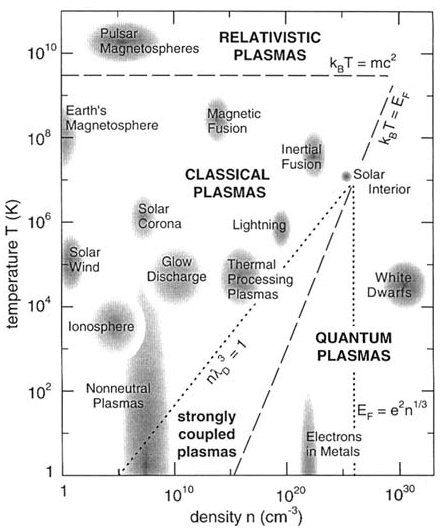
\includegraphics[height=80mm,width=64mm]{figures/1-zoologie.png}{\caption{Classification
de différents plasmas en fonction de $n_e$ et $T_e$ issue du livre du National
Research Council \parencite{NRC}}\label{zoologie}}
\end{figure}

Dans ces plasmas, le degré d'ionisation $\alpha$ est donné par le rapport
entre la densité électronique $n_{e}$ et la densité de gaz neutre
$n_{n}$ :

\begin{equation}
\alpha=\frac{n_{e}}{n_{e}+n_{n}}
\end{equation}

Cette fraction va définir l'importance de l'interaction entre les particules
neutres et les particules chargées. Cependant, même à très faible $\alpha$,
l'apparition d'une population de porteurs de charge va modifier considérablement 
les caractéristiques et la dynamique du plasma.

L'ionisation du gaz suit l'évolution de la température électronique $T_{e}$
qui mesure l'agitation thermique des électrons. Densité et température
électroniques permettent de définir le paramètre plasma:

\begin{equation}
\label{1-paramPlasma}
\Xi=\frac{<E_\text{p}>}{<E_\text{c}>}=\frac{e\puissance{2}
n_{e}\puissance{1/3}}{\varepsilon\indice{0} eT_{e}}
\end{equation}

Le paramètre plasma représente le ratio entre l'énergie thermique des
électrons et leur énergie potentielle électrostatique coulombienne, ie.
l'agitation thermique désordonnée contre les forces d'interactions
coulombiennes structurantes.

Les plasmas classiques (ou cinétiques) sont caractérisés par
$\Xi\ll 1$. Ils ont une population d'électrons assez espacée et/ou une
température suffisamment élevée.

\subsection{Quasineutralité et phénomène d'écrantage}
La dynamique d'un plasma résulte du couplage entre le mouvement des
particules chargées et les forces électromagnétiques présentent ou qui se
forment dans le système :

\begin{equation}
\frac{\text{d} \mathbf
v_\alpha}{\text{dt}}=\frac{q_\alpha}{m_\alpha}(\mathbf E+ \mathbf
v_\alpha\times\mathbf B)
\end{equation}

l'indice $\alpha$ dénotant le type de la particule chargée, $m_\alpha$
et $q_\alpha$ sa masse et sa charge, $\mathbf v_\alpha$ sa vitesse et $(\mathbf
E,\mathbf B)$ le champ électromagnétique.
Elle se décompose principalement sur deux échelles de temps :
la première phase correspond à l'équilibre électrostatique, où une
quasineutralité s'établit au sein du plasma. Dans une deuxième phase, l'évolution quasineutre du
plasma, plus lente, tend à former un équilibre entre le déplacement des particules et la valeur locale
et instantanée des champs de force extérieurs.

L'un des processus les plus rapides que l'on peut trouver dans un plasma est lié à
l'équilibre microscopique électrostatique qui s'opère
entre l'agitation thermique et l'interaction coulombienne des particules. Les
ions et les électrons issus de l'ionisation se réorganisent spontanément pour former un ensemble électriquement neutre.
Cette dynamique est essentiellement portée par les électrons et décrite aux plus petites
échelles spatio-temporelles par le principe fondamental de la dynamique et la loi
de Boltzmann-Poisson :

\begin{align}
\label{1-PFD}
m_{e}\frac{\text{d} \mathbf{v}_{e}}{\text{dt}}=-e\mathbf E
\;\;\;\;\;\;\text{et}\;\;\;\;\;\;
\nabla\cdot\mathbf{E}=\frac{e\,(n_{i}-n_{e})}{\varepsilon\indice{0}}
\end{align}

où $\mathbf{v}_{e}$ est la vitesse de l'électron et
$e\,(n_{i}-n_{e})$ la densité spatiale de charge.
Tout écart à la neutralité, définie par une densité d'ions égale à celle des
électrons, entraîne l'apparition d'un fort champ électrique de rappel à
l'équilibre.
Les échelles fondamentales définies par \eqref{1-PFD} sont la pulsation
plasma et la longueur de Debye, reliée par l'intermédiaire la vitesse thermique :

\begin{equation}
\omega_{pe}\left[\left(\frac{n_e
e\puissance{2}}{\varepsilon\indice{0} m_{e}}\right)^{\text{\textonehalf}}
\right]\cdot\lambda_D\left[\left(\frac{\varepsilon\indice{0}
eT_{e}}{n_e e\puissance{2}}\right)^{\text{\textonehalf}}\right]
=v_{\text{T}{e}}\left[\left(\frac{eT_{e}^{^{\phantom{1}}}}{m_{e}}\right)^{\text{\textonehalf}}\right]
\end{equation}

La pulsation plasma $\omega_{pe}$ correspond à la fréquence typique
d'oscillation des électrons en réponse à une petite séparation de charge. En
conséquence, des processus plus lents que cette fréquence ne voient
apparaître aucun écart à la neutralité.

La longueur de Debye $\lambda_\text{D}$, quant à elle, permet de définir le
phénomène d'écrantage :
C'est une longueur au-delà de laquelle le champ électrique créé par une particule est \emph{écranté} par 
un nuage de particules de charge opposée. Dans un plasma chaque particule est écrantée et participe
à l'écrantage des autres ; le nombre de particules présentes
dans la sphère de rayon $\lambda_\text{D}$ définit alors un paramètre
adimensionné\footnote{Un
grand nombre de particules dans la sphère de Debye $4\pi/3\,n\lambda_D^3\gg1$
définit un plasma idéal, qui peut alors se décrire comme un plasma où le
phénomène d'écrantage électrique est dominant.} semblable au paramètre plasma $\Xi$ \eqrefp{1-paramPlasma}.

Au delà de ces échelles, le plasma est dans un état de \emph{quasineutralité}
\footnote{La quasineutralité n'est pas la seule conséquence de ce phénomène de
réorganisation de charges : lors de l'application d'un champ électrique ou magnétique, celui-ci est rapidement
écranté par le plasma, les particules s'agencent afin de créer un champ
opposé.}, ie. où :

\begin{equation}
n_e=n_i
\label{quasineutralité}
\end{equation}

L'interaction coulombienne d'une particule chargée avec l'ensemble des autres particules peut alors
se réduire à son interaction avec un potentiel électrique local $U$,
résultant de la somme des potentiels microscopiques individuels.

Le système évolue ensuite sur cet équilibre par le biais de
\emph{phénomènes de transport} résultants de l'influence
globale des champs électromagnétiques et de la tendance à
l'homogénéisation du plasma par collisions entres particules.
Ces processus interviennent sur des échelles relativement
lentes et relativement grandes devant $\omega_{p}$ et $\lambda_\text{D}$ :

\begin{equation}
\text{T}\gg \omega_{p}\puissance{-1}
\;\;\;\;\text{et}\;\;\;\;\text{TV}\gg\lambda_\text{D}
\end{equation}

$\text{T}$ étant le temps et $\text{V} $ la vitesse, caractéristiques du
processus de transport considéré.
On parle alors de diffusion/convection de particules, de viscosité (transfert de
quantité de mouvement), de conductivité (transport de charges) ou encore de
conductivité thermique (transport de chaleur).

\subsection{Collisions}
\label{1-Collisions}
En plus de l'interaction coulombienne globale de l'ensemble des espèces chargées, 
les particules, prises deux à deux, peuvent interagir binairement. 
Ces interactions directes entre particules donnent lieu à des transferts
d'impulsion, d'énergie ou encore à des réactions plus complexes telles que
l'ionisation, l'excitation et la recombinaison ; elles sont regroupées
sous le terme général de collisions et se caractérisent par des fréquences de
collisions.

Lors de collisions \emph{élastiques}\footnote{Les collisions sont dites élastiques car
elles donnent lieu à des transferts d'impulsion et d'énergie sans changer
la nature des particules à l'issue de la collision.}, les particules échangent de l'énergie 
en fonction de leur ratio de masse. Entre les électrons et les espèces plus
lourdes, ce transfert d'énergie est très faible et cause une isotropisation
globale des vitesses électroniques.
Dans le cas des plasmas totalement ionisés, seules les collisions coulombiennes 
(interactions binaires entre particules chargées dues à la force de Coulomb)
sont présentes. 
La fréquence de collision $\nu_{ei}$ mesure alors la fréquence à laquelle un
électron est dévié de plus de 90° de sa trajectoire initiale:

\begin{equation}
	\nu_{ei}\sim\frac{4\sqrt{2\pi}e\puissance{4} n_{e} \ln\Lambda
	}{3(4\pi\varepsilon\indice{0})\puissance{2}m_{e}\puissance{1/2}T_{e}\puissance{3/2}}
\end{equation}

avec $\ln \Lambda$ le logarithme de Coulomb,
$\Lambda=\lambda_\text{D}(e\puissance{2}/4\pi\varepsilon\indice{0}
T_{e})\puissance{-1}$ étant le ratio entre la longueur de Debye et une
distance minimale d'approche.

Dans les plasmas faiblement ionisés, le
gaz neutre forme un fond diffus et influence fortement le transport des particules chargées.
Les fréquences de collisions électrons-neutres et ions-neutres sont alors
définies par :

\begin{equation}
	\nu_{en}=\sigma_{en} n_{n} v_{e}
	\;\;\;\;\text{et}\;\;\;\;\nu_{in}=\sigma_{in} n_{n} v_{i}
\end{equation} 
 
avec $\sigma_{en}$ et $\sigma_{in}$ les sections efficaces de
réaction\footnote{\fcolorbox{red}{white}{Les sections efficaces de collisions sont permettent de
caractériser \ldots}} électrons-neutres et ions neutres. La principale
différence dans le transport entre les plasmas faiblement et totalement ionisés tient à la
présence de ce gaz neutre : les collisions avec le gaz sont un puit
direct de quantité de mouvement et d'énergie alors que les
collisions coulombiennes résultent en une redistribution de celles-ci au sein
du plasma.

Les collisions avec le gaz peuvent aussi entraîner des réactions plus complexes
au cours desquelles les particules changent de nature ou d'état (ionisation,
attachement électronique, excitation\ldots).
Ces collisions sont dites \emph{inélastiques} en opposition aux collisions
élastiques. Parmi ces réactions, l'ionisation est le processus le plus
important car il contraint le bilan de particule et contrôle donc l'existence
du plasma. L'association de fréquences de collisions à chaque type de réaction
(eg. $\nu_{iz}$ pour l'ionisation), là aussi en fonction de sections
efficaces, permet un ordering sur l'importance de ces processus dans l'évolution
du plasma.

En plus d'une fréquence, on associe souvent une longueur caractéristique
à l'occurrence d'une collision. Le libre parcours moyen $\lambda_\text{lpm}$
représente alors la distance que peut parcourir une particule à une vitesse
$v_\alpha$ avant de subir une certaine interaction avec le système qui l'entoure
:

\begin{equation}
	\lambda_\alpha=\frac{v_\alpha}{\nu_\alpha}
\end{equation} 

La collisionnalité d'une espèce est
définie par le ratio entre son libre parcours moyen $\lambda_\alpha$ et la
taille $L$ du plasma. Quand le libre parcours moyen est petit devant la
taille du plasma $\lambda_\alpha/L\ll 1$
les particules ont le temps de faire de nombreuses collisions avant de
traverser entièrement le système. Dans des plasmas collisionnels, la description
du transport des espèces est alors simplifiée, les collisions amenant le système dans un état
d'équilibre statistique, caractérisé par des fonctions de distributions de
type Maxwell-Boltzmann (cf. paragraphe \ref{Introduction}-\ref{Maxwell-Boltzmann}).

\fcolorbox{red}{white}{$\sigma$ essentielle à la description
du transport mais difficiles à obtenir\parencite{Phelps}(Phelps)\ldots 
}

$k_{\alpha i}=\left<\sigma_{\alpha i} v_r\right>$
\subsection{Plasma et champ magnétique} 
\label{1-plasma-champMag}
Un plasma magnétisé est un plasma dans lequel le champ magnétique ambiant
$\mathbf{B}$ est suffisamment important pour modifier de manière non-négligeable
le transport des particules. Les plasmas magnétisés sont fortement
anisotropes, réagissant différemment aux forces parallèlement et
perpendiculairement au champ magnétique.

Dans un champ magnétique uniforme, le mouvement d'une particule chargée
soumise à la force de Lorentz peut se décrire par deux composantes :

\begin{itemize}
  \item Un déplacement libre le long lignes de champ
  \item Un mouvement de rotation rapide de la particule
  autour d'un centre-guide dans le plan perpendiculaire à l'axe magnétique
\end{itemize}

Ce mouvement de rotation autour des lignes de champ, appelé mouvement
cyclotronique, est caractérisé par la pulsation cyclotronique : 

\begin{equation}
\omega\indice{{c\alpha}}=\frac{e B}{m_\alpha}
\end{equation}

Le rayon de l'orbite, appelé rayon de Larmor $\rho_{L\alpha}$, révèle quant à
lui une échelle spatiale représentative du transport magnétisé.
Le rayon de Larmor se calcule en fonction de la pulsation cyclotronique et de la vitesse
$v\indice{\alpha}$ de la particule :

\begin{equation}
\rho_{L \alpha}
=\frac{v\indice{\alpha}}{\omega_{c{\alpha}}}
\end{equation}

Pour les ions suffisamment énergétiques, ainsi que pour les électrons en général,
la vitesse typique de la particule est sa vitesse thermique. On peut alors noter :

\begin{equation}
\omega_{c\alpha}\left[\frac{e B}{m_\alpha}\right]
\cdot\rho_{L\alpha}\left[\frac{\sqrt{m_\alpha eT_\alpha}}{eB}\right]
=v\indice{T_{\alpha}}\left[\left(\frac{eT_{\alpha}}{m_{\alpha}}\right)^{\text{\textonehalf}}\right]
\end{equation}

Quand le champ magnétique s'intensifie, les trajectoires
hélicoïdales se resserrent, limitant de plus en plus le déplacement des
particules perpendiculairement à la direction magnétique. L'influence du champ
sur le transport peut alors être mesurée par le paramètre de
magnétisation $\delta$, une espèce pouvant être considérée comme magnétisée à
partir du moment où la longueur caractéristique $L_\perp$ du transport
perpendiculaire considéré est grande devant son rayon de Larmor :

\begin{equation}
\delta=\frac{\rho_{L\alpha}}{L_\perp}\ll 1
\end{equation}

\begin{figure}[htbp]
\centering
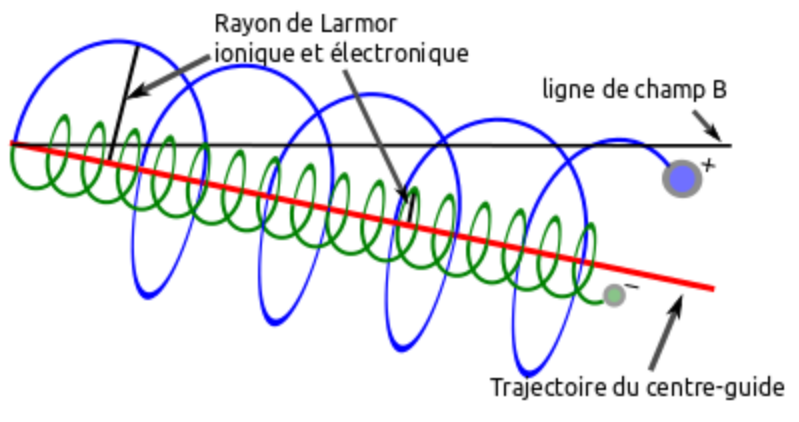
\includegraphics[width=0.8\textwidth]{figures/1-mouvementCyclotron.png}
{\caption{Mouvement cyclotronique des particules autour des lignes de champ
magnétique.}\label{1-particleDrifts}}
\end{figure}

L'application d'un champ électrique conjointement à un champ magnétique
induit une troisième sorte de mouvement, appelé communément "dérive
ExB" (E-cross-B) : le phénomène de dérive se décrit comme un lent déplacement du
centre guide de la particule, perpendiculairement aux champs électrique et
magnétique (cf. figure \ref{1-particleDrifts}). Son expression s'obtient en
prenant le produit vectoriel de l'équation du mouvement par le champ magnétique
:

\begin{equation}
\mathbf{v}_\text{E}=\frac{\mathbf{E}\times\mathbf{B}}{B^2}
\end{equation}

La vitesse de dérive électrique, principale source de transport perpendiculaire
dans un plasma magnétisé, est indépendante de la masse et de la charge des
particules : égale pour les ions et les électrons, elle n'est donc à
l'origine d'aucun courant, ce qui la rend particulière. 

Il peut en effet apparaître d'autres vitesses de dérive. En toute généralité, 
pour chaque force $\mathbf F$ appliquée au plasma, le champ magnétique est à
l'origine d'une vitesse de dérive dans la direction perpendiculaire aux deux
forces qui entrent en jeu :

\begin{equation}
\mathbf{v}\indice{\text{F}}=\frac{\mathbf{F}\times\mathbf{B}}{q_\alpha B^2}
\end{equation}

Si la force $\mathbf F$ est indépendante de la charge ou
fonction de la masse de la particule, la différence entre les vitesses de dérive
électroniques et ioniques induira un courant $\mathbf
j\indice{\text{F}}=en(\mathbf v\indice{\text{F}_\text{i}}-\mathbf
v\indice{\text{F}_\text{e}})$. 

Dans un plasma, où l'anisotropie du champ
magnétique est souvent utilisée pour contrôler et limiter le déplacement des
particules, les vitesses de dérives sont à l'origine d'un transport
 transverse déconfinant, qui s'amplifie généralement par le développement de
 comportements non-linéaires et turbulent.
\subsection{Les gaines électrostatiques}
\label{1-gaines}
Un plasma est souvent, à un moment ou à un autre, amené à entrer en contact avec
une paroi ou un quelconque obstacle matériel. L'interaction entre
les deux milieux conditionne alors l'existence du plasma et influence
fortement son comportement. Une paroi agit en effet comme un parfait
puit de matière et d'énergie pour le plasma, les ions et les électrons se
recombinant facilement à sa surface. Ceci étant, un plasma ne peut se maintenir
que si le nombre de particules créées dans son volume est suffisant pour
balancer ces pertes en surface. 

De plus, les électrons interceptant généralement
plus rapidement la paroi du fait de leur faible masse et de leur température,
polarisent négativement la surface du matériau.
L'augmentation progressive de ce potentiel mène alors à la formation en périphérie du plasma d'une région de densité ionique
supérieure, et donc non-neutre, que l'on appelle gaine électrostatique (ou gaine de Debye, voir
figure~\ref{1-gaine1}). Cette gaine a une taille caractéristique de l'ordre de
quelques longueurs de Debye $\lambda_\text{D}$, longueur critique à partir de
laquelle un plasma quasineutre  s'écrante de la paroi.

\begin{figure}[htbp]
\centering
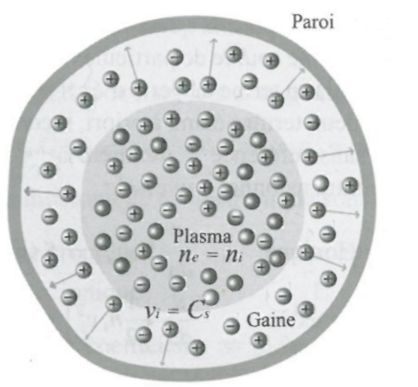
\includegraphics[height=60mm,width=60mm]{figures/1-sheath.jpg}{\caption{Séparation
du plasma entre une région quasineutre et la gaine à sa
périphérie. A la frontière, il y a rupture de la quasineutralité et la vitesse
ionique est égale à la vitesse de Bohm
$c_\text{s}$\parencite{Rax}.}\label{1-gaine1}}
\end{figure}

Dans les plasmas classiques où la taille de la gaine est petite
à l'échelle du plasma, son rôle est essentiellement de
maintenir la quasineutralité dans le volume en régulant les flux d'ions et
d'électrons tombant aux parois. Les électrons, énergétiquement confinés par le
potentiel de la surface, forment un équilibre électrostatique à l'intérieur du
plasma, et peuvent donc être décrits par une distribution de Boltzmann :

\begin{equation}
	n_{e}=n\indice{0}\exp(eU/eT_{e})
\end{equation}

avec $n\indice{0}$ la densité de référence prise au niveau du potentiel nul.
Pour égaler le flux électronique et écranter la polarisation de la paroi, la
quasineutralité doit être brisée. L'étude de la transition plasma-gaine montre,
à travers l'énoncé du critère de Bohm \parencite{Stangeby}, que
cette condition ne peut être remplie que si la vitesse ionique en entrée de
gaine est au moins égale à $c_s$, communément appelée vitesse de Bohm ou encore
vitesse acoustique ionique\footnote{la deuxième appellation provient de la similitude entre la
transition subsonique-supersonique qui s'observe dans les gaz neutres. Les
ondes acoustiques, reliées aux surpressions et aux sous-pressions, se propagent
dans un plasma par le champ électrique. L'élasticité du plasma est alors due à
la température électronique $T_\text{e}$ et à l'inertie ionique.} :

\begin{equation}
c_s=\sqrt{\frac{e (T_{e}+T_{i})}{m_{i}}}
\end{equation}

\subsubsection{Physique de la gaine}
\label{1-gaine}
Considérons de nouveau l'équation de Poisson, qui contrôle l'évolution du
potentiel électrique, au voisinage de la paroi :
\begin{equation}
\frac{d\puissance{2}\Phi}{d\xi}=\frac{1}{\lambda_D\puissance{2}}\frac{n_{e}-n_{i}}{n\indice{0}}
\end{equation}
 où $\Phi$ est le potentiel normalisé $\Phi=eU/T_{e}$, $\xi$ est la
 direction normale à la paroi, $n_{e}$ et $n_{i}$ les densités
 électronique et ionique respectivement, et $n\indice{0}$ la densité
 moyenne du plasma. Quand le plasma est suffisamment dense pour que $\lambda_D\ll
 L$, l'équation de poisson permet d'estimer le champ électrique des deux
 régions :

 \begin{itemize}
   \item Face à la paroi chargée négativement se
   développe un fort gradient de potentiel ($d\Phi/d\xi\sim 1/\lambda_D$) dont le plasma
   s'écrante en formant une épaisseur de peau ionique non-neutre de
   taille caractéristique $\lambda_D$
   \item Le reste du plasma, de taille caractéristique $L$, satisfait
   à l'hypothèse de quasineutralité et le potentiel varie en
   $d\Phi/d\xi\sim1/L$
 \end{itemize}

La frontière entre la gaine et la partie
quasineutre du plasma, qualifiée de prégaine, peut être définie à partir de la
brisure de la quasineutralité. A l'intérieur de la gaine, afin de maintenir la
décroissance du potentiel jusqu'à la paroi, la densité ionique doit diminuer
moins rapidement que la densité d'électrons. 

\begin{equation}
	\frac{dn_{i}}{d\xi}<\frac{dn_{e}}{d\xi}
\end{equation}

En appliquant la loi de conservation de l'énergie entre
l'entrée de la gaine (où les densités sont égales) et la paroi, on trouve le
critère général obtenu par Bohm en hydrodynamique :

\begin{equation}
	v_{{i}\,|_{\xi=\xi_s}}\geq c_{s}
\end{equation}

où $\xi_s$ indique la position de la frontière plasma/gaine.
Dans le cas de plasmas non-magnétisés et avec l'hypothèse d'une température
électronique uniforme $T_{e}\gg T_{i}$, on montre de plus que la
vitesse ionique doit rester subsonique dans la prégaine, donnant une limite dure
$v_{i}=c_{s}$.
Pour estimer la chute de potentiel, on peut alors écrire :

\begin{equation}
	\left(\frac{2e(\Phi_{\xi}-\Phi_{\xi_{s}})}{m_{i}}+v_{i}\puissance{2}\right)_{\xi=\xi_s}=
	\frac{eT_{e}}{m_{i}}=\left(\frac{2e(\Phi_{\xi}-\Phi_{\xi_{s}})}{m_{i}}\right)_{\xi=0}
\end{equation}

A partir d'une région centrale où $v_{i}=0$, le potentiel chute donc de
$T_{e}/2$ et la densité, par conséquence, d'un facteur
$n_{s}/n\indice{0}=e^{-1/2}$, l'indice $s$ dénotant dans la suite du
paragraphe la position de la gaine.
Le flux d'électron atteignant la paroi se calcule en intégrant une maxwellienne sur le
demi-espace des vitesses positives :

\begin{equation}
	v_{e}^\text{wall}=\frac{1}{\sqrt{\pi}v_{e\perp}}\int_0^\infty
	v_{e\perp}
	e^{-v_{e\perp}^2/v_{\text{T}e}^2}dv_{e\perp}=\frac{1}{2\sqrt{\pi}}v_{\text{T}e}=\sqrt{\frac{eT_{e}}{2\pi
	m_{e}}}
\end{equation}

les flux ionique et électronique sont égaux à la paroi, le flux ionique étant
conservé à travers la gaine :

\begin{equation}
	\Gamma_{e}^\text{wall}=n_{e}^\text{wall}\exp{\left(\frac{\Phi_\text{wall}}{T_{e}}\right)}\sqrt{\frac{eT_{e}}{2\pi
	m_{e}}}=\Gamma_{i}^\text{wall}=\Gamma_{i}
\end{equation}
\begin{equation}
\label{1-densitéIonique}
	n_{i}=n_{s}\exp{\left(\frac{\Phi_{s}-\Phi_\text{wall}}{T_{e}}\right)}\sqrt{\frac{eT_{e}}{2\pi
	m_{e}v_{i}\puissance{2}}}
\end{equation}

en prenant la relation \ref{1-densitéIonique} au seuil de la gaine, on peut
calculer le potentiel flottant $\Lambda$ qui s'établit naturellement entre le
plasma et le mur :

\begin{equation}
	\Lambda=\Phi_{s}-\Phi_\text{wall}=\frac{1}{2}T_{e}\ln{\frac{m_{i}c_{s}^2}{2\pi
	m_{e}v_{i}\puissance{2}}}
	\end{equation}

Si l'on suppose donc $v_\text{i}=c_{s}$ à l'entrée de gaine, le potentiel
flottant d'un plasma d'hydrogène à une température électronique d'1eV est
défini par le logarithme du rapport de masse :

\begin{equation}
	\Lambda=\frac{1}{2}\ln{\frac{m_{i}}{2\pi
	m_{e}}}=2.8388
	\end{equation}

Pour résumer ces considérations, les profils de densité,
potentiel et vitesse ionique pour un plasma collisionnel sont tracés sur la
figure (\ref{1-profilesgaine}) :
	
\begin{figure}[htbp]
\centering
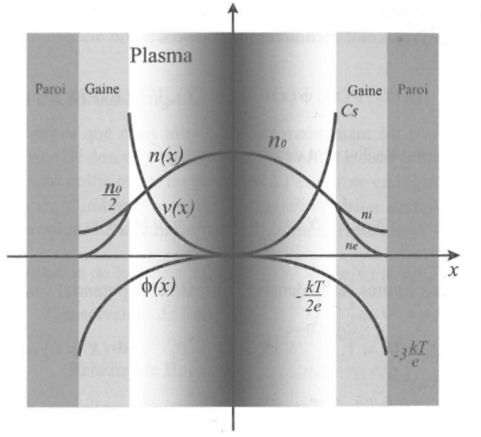
\includegraphics[height=70mm,width=80mm]{figures/1-sheathprofiles.jpg}{\caption{Profils
des densités électronique, ionique,
du potentiel et de la vitesse ionique à
la transition plasma-gaine\parencite{Rax}. La taille
de la gaine est ici exagérée.}\label{1-profilesgaine}}
\end{figure}

$\Lambda$ est le potentiel correspondant à une égalité stricte des flux au
niveau de la gaine. Cependant, il ne définit qu'une position
d'équilibre autour de laquelle le potentiel s'ajuste constamment pour
équilibrer les flux à travers la circulation des courants de gaines :

\begin{equation}
	j_{s}=en_{s}v_{i}\left(1-e^{\Lambda-\Phi_{s}/T_{e}}\right)
\end{equation}

\fcolorbox{red}{white}{
\begin{minipage}{0.9\textwidth}flux d'énergie et de chaleur\ldots?
\end{minipage}}

\subsubsection{Gaine dans les plasmas magnétisés}
La situation dans le cas d'un champ magnétique normal à la paroi est
identique au cas non-magnétisé. La théorie peut de plus être étendue 
à une incidence $\alpha_\text{inc}$ non-rasante des lignes de champ où une
prégaine magnétique de quelques rayons de Larmor accélère les ions jusqu'à la
vitesse de Bohm via une déflexion imposée à la trajectoire des particules. Le
critère de Bohm est alors légèrement corrigé pour tenir compte du transport transverse
\cite{Stangeby} :

\begin{equation}
	v_\para\geq
	c_{s}-\frac{v_\perp}{\tan{\alpha_\text{inc}}}
\end{equation}
 
 $v_\perp$ désignant la composante de la vitesse ionique perpendiculaire à la
 surface. La valeur critique de vitesse parallèle est donc
 diminuée en fonction de l'importance de la vitesse des dérives. Le cas
 d'une gaine totalement parallèle au champ magnétique s'avère bien plus complexe
 et n'est pas clairement défini dans la littérature.

\section{Fonction de distribution et théorie fluide}
\label{Maxwell-Boltzmann}

Le plasma est un système dynamique complexe dont l'évolution au cours du temps
peut être suivie de différentes façons. La description la plus complète utilise
une approche statistique dans laquelle chaque espèce $\alpha$ est caractérisée
par une fonction de distribution $f_\alpha(\mathbf{r},\mathbf{v},t)$
représentant le nombre moyen de particules occupant un volume infinitésimal
de l'espace des phases à un instant $t$. Son évolution est alors décrite à
travers l'équation de Boltzmann.

Sur des échelles de temps suffisamment longues, l'évolution d'un plasma est 
essentiellement due à des processus de transport macroscopiques pour lesquels
une description fluide est plus adaptée. Une espèce est alors
caractérisée par un ensemble de paramètres macroscopiques, calculés à
partir des moments de la fonction de distribution. Les plus importants -
la densité $n_\alpha$, la vitesse fluide $u_\alpha$ et la température $T_\alpha$
- ont des interprétations physiques immédiates et sont souvent mesurables
expérimentalement. L'évolution de ces quantités est ensuite décrite par les
équations fluides, obtenues en prenant les moments correspondants de l'équation de Boltzmann.

\subsection{L'équation de Boltzmann}
Le nombre de particules dans un plasma étant généralement élevé, il est
approprié de les représenter en fonction de chaque
espèce\footnote{La fonction de
distribution peut aussi servir à suivre les différents états quantiques des
ions, des atomes et des molécules (rotationnel, vibrationnel, électronique).}
d'une manière statistique par une fonction de
distribution $f_\alpha$ dénombrant le nombre moyen de particules présentes à un
instant $t$ dans un volume de l'espace des phases, ie. $f_\alpha(\mathbf
r,\mathbf v,t)\text{d}\puissance{3}\mathbf r\text{d}\puissance{3}\mathbf v$.
L'évolution de cette fonction de distribution sous l'influence des forces
extérieures et des collisions est alors décrite par l'équation cinétique de
Boltzmann :

\begin{equation}
\label{1-BoltzmannEquation}
\partial_tf_\alpha+\mathbf{v}_\alpha\cdot\vec\nabla_\mathbf{r}f_\alpha+
\frac{\mathbf{F}}{m_\alpha}\cdot\vec\nabla_{\mathbf{v}}f_\alpha
=C[f_\alpha]
\end{equation}

où $\vec\nabla$ est l'opérateur gradient appliqué à l'espace des positions ou
des vitesses, et $\mathbf{F}$ la somme des forces extérieures, qui se résument
souvent aux forces électromagnétiques. Lors de collisions, les particules peuvent changer de
trajectoire, et ainsi se déplacer instantanément dans des régions éloignées de leur espace des
phases (ou encore totalement disparaître lors de collisions inélastiques).
L'opérateur de collisions $C[f_\alpha]$, qui doit représenter l'intégralité de
ces effets discrets, se réécrit généralement comme une somme sur l'ensemble des
espèces de coefficients spécifiques à chacune des interactions.

L'équation de Boltzmann permet de suivre
parfaitement l'évolution de l'ensemble des espèces du plasma et elle est
même parfois incontournable pour décrire avec exactitude les interactions
ondes-particules ou celles impliquant des particules rapides. 

Cependant, \eqref{1-BoltzmannEquation} est très
difficile à résoudre du fait de la complexité de l'opérateur de collisions
$C[f]$. Les méthodes utilisées pour la résoudre nécessitent de nombreuses
approximations sur la fonction de distribution\parencite{HagelaarHDR}. Pour
réduire le problème, l'équation peut être intégrée dans l'espace des vitesses
en ne gardant que les dimensions statiales et temporelle du système : c'est
l'approche fluide.

\subsection{Les quantités fluides}
L'approche fluide consiste à décrire le comportement des particules de chaque
espèce en terme de quantités macroscopiques moyennes telles que la densité $n$,
la vitesse moyenne $\mathbf u$ et la température $T$. Ces quantités sont dérivées
des moments des fonctions de distributions sur l'espace des vitesses.
Pour une espèce $\alpha$ le moment en vitesse d'ordre $k$ est un tenseur d'ordre
$k$ :

\begin{equation}
\mathbf M^{(k)}_\alpha(\mathbf
r,t)=\int\mathbf{v} \mathbf{v} . . .
\mathbf{v} f_\alpha(\mathbf r,\mathbf v,t)
\,\text{d}\puissance{3}\mathbf{v}
\end{equation}

Les trois premiers moments $\mathbf M^{(0)}$, $\mathbf M^{(1)}$ et $\mathbf
M^{(2)}$ ont chacun un nom et une interprétation physique simple. La densité
$n_\alpha$, qui mesure le nombre de particules de l'espèce $\alpha$ dans un
petit volume, et le flux de particule $\boldsymbol{\Gamma_\alpha}$, qui
s'exprime en fonction de la vitesse fluide $\mathbf u_\alpha$, sont
donnés par :

\begin{equation}
n_\alpha(\mathbf
r,t)=\int f_\alpha(\mathbf r,\mathbf v,t)
\,\text{d}\puissance{3}\mathbf{v}
\end{equation}

\begin{equation}
\boldsymbol{\Gamma}_\alpha(\mathbf
r,t)=n_\alpha\mathbf u_\alpha=\int \mathbf v f_\alpha(\mathbf r,\mathbf
v,t) \,\text{d}\puissance{3}\mathbf{v}
\end{equation}

Le moment d'ordre deux (le tenseur de pression) est mesuré dans le repère au
repos du fluide en introduisant la vitesse relative $\mathbf w=\mathbf
v-\mathbf u_\alpha$ : 

\begin{equation}
\mathbf P_\alpha(\mathbf
r,t)=m_\alpha\int \mathbf w\mathbf w
f_\alpha(\mathbf r,\mathbf v,t) \,\text{d}\puissance{3}\mathbf{v}
\end{equation}

le tenseur de pression mesure l'écart quadratique entre la vitesse moyenne des
particules et la vitesse fluide. On introduit ensuite la
pression scalaire $p_\alpha$ et le tenseur de viscosité
$\boldsymbol{\Pi}_\alpha$, tels que:

\begin{equation}
\label{1-tenseurPression}
\mathbf P_\alpha=p_\alpha\,\mathbf I + \boldsymbol{\Pi}_\alpha
\end{equation}

avec $\mathbf I$ la matrice identité. Par analogie avec la théorie fluide
conventionnelle, on s'attend à ce que les termes diagonaux soient dominants
quand l'espèce est à l'équilibre thermique. La trace du tenseur
$\mathbf P_\alpha$, quantifie ainsi la densité d'énergie cinétique
interne de l'espèce et peut se réécrire en définissant la température partielle 
$T_\alpha$ mesurée en unité d'énergie:

\begin{equation}
\frac{3}{2}p_\alpha=\frac{3}{2}n_\alpha eT_\alpha=\frac{m_\alpha}{2}\int 
w\puissance{2} f_\alpha(\mathbf r,\mathbf v,t) \,\text{d}\puissance{3}\mathbf{v}
\end{equation}

En montant en ordre, les moments apportent de plus en plus de détails sur la
fonction de distribution, donnant théoriquement une description du plasma
strictement équivalente à la description statistique. Dans les fluides
collisionnels, il ne suffit généralement que de la densité $n_\alpha$, de la
vitesse $\mathbf{u}_\alpha$ et de la température $T_\alpha$ pour caractériser
l'ensemble des particules d'une espèce.



\subsection{Les équations de conservation}

A chaque quantité macroscopique est adjointe une équation traduisant sa
conservation. Ces équations de conservation, aussi appelées équations fluides,
sont obtenues en prenant les moments correspondants de l'équation de Boltzmann.

\subsubsection{Conservation de la matière}
L'équation de conservation de la matière contrôle
l'évolution de la densité. On l'obtient en intégrant
l'équation de Boltzmann (\eqref{1-BoltzmannEquation}) sur l'espace des
vitesses~:

\begin{equation}
\label{1-eqContinuite}
	\partial_tn_\alpha+
	\nabla\cdot\left(n_\alpha\mathbf{u_\alpha}\right)=S_\alpha
\end{equation}

avec $n_\alpha$ la densité de l'espèce, $\mathbf{u_\alpha}$ la vitesse
fluide et $S_\alpha$ un terme source se mesurant en nombre de particules par
unité de temps et de volume. Dans les plasmas froids, ce terme source est issu
de l'intégration du terme de collisions et rend compte du nombre de particules
créées ou perdues lors de collisions inélastiques. Il est constitué
par l'ensemble des intéractions collisionnelles et chimiques :
$$S_\alpha=\sum_s N_s n_{\alpha}n_{s}k_{\alpha s}$$ où $s$ denote les autres
espèces présentes dans le plasma, $N$ est le nombre de particules créées lors
d'une collision (négatif en cas de destruction), $n_i$ la densité de l'espèce en collision et $k_{\alpha s}=\left<\sigma_{\alpha s}
v_r\right>$ le coefficient de collision/réaction
associé (cf.\S\ref{1-Collisions}), avec $v_r=(\mathbf u_s-\mathbf u_\alpha)$
la vitesse relative des deux fluides.

\subsubsection{Conservation de la quantité de mouvement}
L'équation de conservation de la quantité de mouvement peut être considérée
comme le moment d'ordre un en vitesse de l'équation de Boltzmann. En multipliant
\eqref{1-BoltzmannEquation} par $\mathbf v$ puis en intégrant sur l'espace des
vitesse, on obtient :

\begin{equation}
\label{1-eqQuantiteMouvement}
\partial_t m_\alpha n_\alpha \mathbf{u}_\alpha + 
\nabla\cdot\left(m_\alpha n_\alpha
\mathbf{u}_\alpha\mathbf{u}_\alpha+\mathbf{P_\alpha}\right)=q_\alpha
n_\alpha\left(\mathbf E+\mathbf u_\alpha\times\mathbf B\right)
+\mathbf{R_\alpha}
\end{equation}

avec $\mathbf{P_\alpha}$ le tenseur de pression, $\mathbf{E}$ et $\mathbf{B}$
les forces électromagnétiques et $\mathbf{R_\alpha}$ un terme de
friction traduisant la perte et l'échange de quantité de mouvement dans les
collisions. En toute généralité, on peut écrire ce transfert de quantité de
mouvement pour chaque espèce $\alpha$ comme une somme de deux composants :
\begin{equation}
\mathbf{R_\alpha}=\sum_{s\neq\alpha}(\mathbf{R}_{\alpha s}^{(\mathbf
u)}+\mathbf{R}_{\alpha s}^{(T)})
\end{equation}
Le terme
$\mathbf{R}_{\alpha i}^{(T)}$ est connu sous le nom de force thermique et
émerge de la dépendance en vitesse des fréquences de collisions. Le terme
$\mathbf{R}_{\alpha i}^{(\mathbf u)}$ est une force de frottement
proportionnelle à la vitesse relative des espèces en collision :
\begin{equation}
\mathbf{R}_{\alpha}^{(\mathbf
u)}=n_\alpha\sum_{s\neq\alpha}\frac{m_\alpha m_s}{m_\alpha+m_s}
n_sk_{\alpha s} \left(\mathbf u_s-\mathbf u_\alpha\right)
\end{equation}

Dans le cas de plasmas fortement ionisés où les collisions coulombiennes sont
dominantes, $\mathbf{R_\alpha}$ s'exprime à travers la fermeture de
Braginsky en fonction du courant $\mathbf
j=en\left(\mathbf u_i-\mathbf u_e\right)$ et du gradient de température
électronique $\nabla T_e$~\parencite{Braginsky}. Dans le cadre des plasmas
froids, c'est les collisions avec le gaz au repos qui sont dominantes. La force termique peut être
négligée et le terme de friction se réécrit de façon macroscopique :
\begin{equation}
\label{1-forceFriction}
\mathbf{R_{\alpha}}=\mathbf{R_{\alpha}^{(\mathbf
u)}}=m_\alpha n_\alpha\mathbf u_\alpha\sum_{s\neq\alpha}\frac{m_s}{m_\alpha+m_s}
n_sk^m_{\alpha s} = m_\alpha n_\alpha \nu_\alpha \mathbf u_\alpha
\end{equation}
où $k^m_{\alpha s}=\left<\sigma^m_{\alpha s}v_r\right>$ est un coefficient
efficace de transfert de quantité de mouvement. En remplacant les expressions du
tenseur de pression (\eqref{1-tenseurPression}) et du terme de friction (\eqref{1-forceFriction}) dans
\eqref{1-eqQuantiteMouvement} et en la combinant avec l'équation de continuité
(\eqref{1-eqContinuite}), on obtient l'équation du mouvement qui contrôle
l'évolution de la vitesse :

\begin{equation}
\label{1-eqMouvement}
\partial_t \mathbf{u}_\alpha + (\mathbf{u}_\alpha\cdot\nabla)\mathbf{u}_\alpha
+\left(\nu_\alpha+\nu_{iz}\right) \mathbf
u_\alpha=\frac{q_\alpha}{m_\alpha}\left(\mathbf E+\mathbf u_\alpha\times \mathbf
B\right) -\frac{\nabla p_\alpha}{m_\alpha n_\alpha} -\frac{\nabla\cdot\boldsymbol{\Pi}_\alpha}{m_\alpha n_\alpha}
\end{equation}

où $\nu_{{iz}}=S_\alpha/n_\alpha$ provient de la substitution de l'équation
de continuité et caractérise la perte effective de quantité de mouvement
dans les collisions inélastiques : les particules sont ionisées sans
vitesse initiale et perdues à la vitesse moyenne $\mathbf u_\alpha$, entraînant une force de traînée nette
proportionnelle à la vitesse du fluide en mouvement $\mathbf
F_{\text{drag}}=\mathbf{u_\alpha}\nu_{{iz}}$.

\subsubsection{Conservation de l'énergie}
Le deuxième moment de l'équation de Boltzmann donne une équation tensorielle
dont la contraction garantit la conservation de l'énergie moyenne du système.
L'équation de conservation de
l'énergie, qui s'obtient également en multipliant \eqref{1-BoltzmannEquation}
par $m_\alpha {u}_\alpha^2/2$, s'écrit :

\begin{equation}
\label{1-eqEnergie}
\partial_t \varepsilon_\alpha+
\nabla\cdot\left(\varepsilon_\alpha\mathbf{u}_\alpha+\mathbf
P_\alpha\cdot\mathbf{u}_\alpha + \mathbf q_\alpha\right) =q_\alpha
n_\alpha\mathbf E\cdot
\mathbf{u}_\alpha+Q_\alpha
\end{equation}

où $\varepsilon_\alpha=m_\alpha n_\alpha u_\alpha^2/2+3p_\alpha/2$ est
la densité d'énergie du fluide. L'équation fait intervenir le troisième moment
de la fonction de distribution, $$\mathbf q_\alpha=m_\alpha
n_\alpha\left<w^2\mathbf w\right>/2$$ qui représente le flux de chaleur
(d'énergie chaotique), ie. le flux d'énergie dans le repère au repos du fluide. 
Enfin, $Q_\alpha$ est la production \emph{totale}\footnote{Dans de nombreux ouvrages, le terme de chauffage
collisionnel est décomposé en un terme de chauffage dirigé et un terme mesurant
le chauffage dans le repère au repos $\text{W}_\alpha$: $$Q_\alpha=\int_{\mathbf
v}\frac{m_\alpha}{2}v_\alpha^2C_\alpha d\mathbf v=\int_{\mathbf
v}\frac{m_\alpha}{2}(u_\alpha+w_\alpha)^2C_\alpha d\mathbf
v\sim\text{W}_\alpha+\mathbf u_\alpha\cdot\mathbf R_\alpha $$ Après le travail
algébrique sur les équations pour obtenir la conservation de l'énergie
thermique, le terme $\mathbf u_\alpha\cdot\mathbf R_\alpha$ disparaît pour
ne laisser que le terme $\text{W}_\alpha$. 

Dans ce manuscrit, nous
considérons dans les équations la perte d'énergie totale ; le terme de
chauffage par friction (ie. l'effet Joule) est donc toujours présent après la
substitution dans l'équation d'énergie.} de chaleur lors de collisions et de
réactions chimiques.
Pour les électrons, cette puissance collisionnelle est généralement négative et peut s'exprimer en terme de taux:
\begin{equation}
	Q_e=\int_{\mathbf
	v}\frac{m_\alpha}{2}v^2C_\alpha d\mathbf
	v=-en_e\sum_{s}\left(E_sn_sk_s+\frac{2m_e}{m_s}k^m_s\varepsilon_e\right)
\end{equation}

avec $E_s$ l'énergie de seuil de la réaction. On peut maintenant soustraire la
contribution de l'énergie dirigée $\text{U}_{\alpha}=m_\alpha n_\alpha
u_\alpha^2/2$ de \eqref{1-eqEnergie} en utilisant le produit scalaire de l'équation de
conservation de la quantité de mouvement (\eqref{1-eqQuantiteMouvement}) et de
la vitesse fluide pour obtenir une équation de conservation sur l'énergie
interne (thermique) d'une espèce :

\begin{equation}
\label{1-eqEnergieInterne}
\frac{3}{2}\partial_t p_\alpha + 
\nabla\cdot\left(\frac{3}{2}p_\alpha
\mathbf{u}_\alpha+\mathbf q_\alpha\right)+p_\alpha\nabla\cdot\mathbf u_\alpha
+\boldsymbol{\Pi}_{\alpha j k}\frac{\partial u_{\alpha j}}{\partial{x_k}} =
{Q_\alpha}+(2n_\alpha\nu_\alpha+S_\alpha)\text{U}_\alpha
\end{equation}

Dans cette équation, $p_\alpha\nabla\cdot\mathbf u_\alpha$ représente la
puissance produite par la pression partielle qui résulte du
refroidissement/chauffage lié à la compression ou à l'expansion d'un volume de
plasma et le terme $\boldsymbol{\Pi}_{\alpha j k}\partial u_{\alpha
j}/\partial{x_k}$ décrit le chauffage visqueux. Le terme
$(2n_\alpha\nu_\alpha+S_\alpha)\text{U}_\alpha$ apparaît distinctement comme une
production ou une perte de chaleur conséquente du travail de la force de traînée générée par
les collisions. C'est un terme primordial pour capturer correctement le
comportement de la température électronique dans les plasmas froids. 

En utilisant l'équation de
continuité pour réduire l'équation d'énergie (\eqref{1-eqEnergieInterne}), on
obtient une équation d'évolution pour la température de l'espèce :

\begin{equation}
\label{1-eqTemperature}
\frac{3}{2}n_\alpha\frac{\text{d}eT_\alpha}{\text{dt}}+\nabla\cdot\mathbf
q_\alpha + p_\alpha\nabla\cdot\mathbf u_\alpha +\boldsymbol{\Pi}_{\alpha j
k}\frac{\partial u_{\alpha j}}{\partial{x_k}}+ \frac{3}{2}S_\alpha eT_\alpha =
{Q_\alpha}+(2n_\alpha\nu_\alpha+S_\alpha)\text{U}_\alpha
\end{equation}

avec $\text{d}/\text{dt}=\partial_t+\mathbf u\cdot\nabla$ la notation de
la dérivée convective. En substituant enfin le terme de compression
$p_\alpha\nabla\cdot\mathbf u_\alpha$ pour faire disparaître la divergence de la vitesse,
\eqref{1-eqTemperature} se réécrit :

\begin{equation}
\label{1-eqTemperature2}
\frac{3}{2}n_\alpha\frac{\text{d}eT_\alpha}{\text{dt}}+\nabla\cdot\mathbf
q_\alpha +\boldsymbol{\Pi}_{\alpha j k}\frac{\partial u_{\alpha
j}}{\partial{x_k}}+ \frac{5}{2}S_\alpha eT_\alpha = eT_\alpha\frac{\text{d}n_\alpha}{\text{dt}}+ 
{Q_\alpha}+(2n_\alpha\nu_\alpha+S_\alpha)\text{U}_\alpha
\end{equation}

Dans notre étude des plasmas froids magnétisés, la température ionique $T_i$
est très proche de celle des neutres et il n'est pas nécéssaire de décrire
son évolution. $T_e$ en revanche joue un rôle primordial dans le comportement
du plasma car directement responsable de l'ionisation du gaz et donc du
transport collisionnel généré. Comme le flux de chaleur électronique est très
sensible au champ magnétique et tend à influencer de façon notable le
comportement de $T_e$, il doit être décrit avec attention à travers une équation
spécifique.

\subsubsection{Conservation de la chaleur électronique}

Les équations \eqref{1-eqEnergieInterne}-\eqref{1-eqTemperature2} font
intervenir des moments d'ordre trois, les composantes du vecteur de flux de
chaleur $\mathbf q_\alpha$ dont les expressions sont assez similaires et se
dérivent de la même façon que celles du flux de particules. Quand les électrons
sont suffisement collisionnels et que l'énergie dirigée est inférieure à
l'énergie chaotique ($m_eu_e^2/2\ll T_e$), l'équation pour le flux de chaleur
électronique prend la forme~\parencite{Golant} :

\begin{equation}
\label{1-eqFluxChaleur}
\partial_t\mathbf
q_e+\frac{5}{2}\frac{n_e
T_e}{m_\alpha}+\frac{e}{m_e} \mathbf q_e\times\mathbf
B=\frac{\delta\mathbf q_e}{\delta t}
\end{equation}


En considérant le faible ratio de
masses et en supposant que la chaleur est essentiellement perdue lors des
collisions avec les neutres, on trouve une expression pour le terme de collision  $\delta\mathbf q_e/\delta
t$ qui est alors
proportionnel à la fréquence de collision $\nu_{en}$. \eqref{1-eqFluxChaleur} se
réécrit :

\begin{equation}
\label{1-eqFluxChaleur2}
\partial_t\mathbf
q_e+\frac{5}{2}\frac{n_e
T_e}{m_\alpha}+\frac{e}{m_e} \mathbf q_e\times\mathbf
B=-\nu_{en}\mathbf q_e
\end{equation}

Le système (\eqref{1-eqContinuite}, \eqref{1-eqQuantiteMouvement},
\eqref{1-eqEnergieInterne},\eqref{1-eqFluxChaleur}) forme une suite d'équations
de conservation décrivant le comportement des espèces dans le plasma.
Ces équations sont valides pour des échelles de temps et d'espace grandes devant
les échelles caractéristiques collisionnelles :
\begin{equation}
\text{T}\gg \nu_{\alpha}\puissance{-1}
\;\;\;\;\text{et}\;\;\;\;\text{L}\gg\lambda_\alpha=\frac{c_s}{\nu_\alpha}
\end{equation}
ie. quand les fonctions de distributions se
rapprochent de maxwelliennes locales\footnote{Il suffit de deux vitesses pour caractériser
une maxwellienne, la vitesse moyenne $\left<v\right>$ et la vitesse quadratique moyenne
$\sqrt{\left<v\puissance{2}\right>}$ :
$$
	\left<v\right>=\sqrt{\frac{8eT}{\pi m}} \;\;\;\;\text{et}\;\;\;\; 
	\left<v\puissance{2}\right>=\frac{3eT}{m}
$$ Les moments de la fonction de distribution se calculent ainsi facilement.}:
\begin{equation}
\label{1-MaxwellDistribution}
	f_\alpha\simeq n_\alpha
	\left(\frac{m_\alpha}{2\pi
	eT_\alpha}\right)\puissance{3/2}4\pi
	u_\alpha\puissance{2}\exp\left(\frac{-m_\alpha \left(\mathbf
	v_\alpha-\mathbf u_\alpha\right)\puissance{2}}{2eT_\alpha}\right)
\end{equation}

Il peut sembler qu'une description fluide d'un plasma soit fortement limitée
par cette hypothèse. Cependant, excepté pour les interactions
ondes-particules, elle est valide et suffisante dans de nombreuses
situations : les électrons sont généralement en équilibre de Boltzmann et une
description cohérente du flux ionique peut être obtenue en considérant l'hypothèse de quasineutralité du
plasma.

\section{Modèles pour le transport magnétisé}

La théorie fluide, en supposant une cohésion macroscopique de l'ensemble des
particules, fournit une description de base pour étudier les phénomènes de
transport dans les plasmas. A partir de ce formalisme, la plupart des modèles
sont construits en simplifiant les équations pour ne retenir que les
caractéristiques et processus essentiels du système à étudier. 

La première hypothèse communément retenue pour simplifier le modèle consiste à
considérer le tenseur de pression isotrope, ie.
$\boldsymbol{\Pi}_\alpha=0$, en supposant que les tranferts d'impulsion dus
aux collisions entre particules d'espèces différentes ont plus d'effet que
ceux résultants de la viscosité. L'équation du
mouvement~\eqref{1-eqMouvement} se réduit ainsi à un équilibre entre les forces
d'inertie, de traînée, de Lorentz et de pression :

\begin{equation}
\label{1-eqBilanForce}
\underbrace{m_\alpha n_\alpha\left(\partial_t \mathbf{u_\alpha} +
(\mathbf{u_\alpha}\cdot\nabla)\mathbf{u_\alpha}\right)}_\text{Inertie}
+\underbrace{m_\alpha n_\alpha\nu_\alpha\mathbf
u_\alpha}_\text{Traînée}=\underbrace{{q_\alpha n_\alpha}\left(\mathbf E+\mathbf
u_\alpha\times \mathbf B\right)}_\text{Forces électromagnétiques}
-\underbrace{{\nabla p_\alpha}}_\text{Pression}
\end{equation}
 
Le poids des différents termes de \eqref{1-eqBilanForce} varie en fonction des
paramètres du plasma et permet de définir le type d'écoulement des fluides
électroniques et ioniques. En mécanique des fluides, l'habitude est de définir
des nombres adimentionnés, dérivant des ratios entre les termes d'inertie, de
pression et de traînée, pour caractériser le fluide : ce sont les nombres de
Mach, de Reynolds et de Knudsen.

En physique des plasmas les fluides électroniques et ioniques sont couplés à
travers le champ électrique et le champ magnétique rend le transport très
anisotropique. Bien que l'on puisse dériver ici aussi des nombres
adimentionnés pour certains phénomènes tels que la transition
subsonique-supersonique, la catégorisation des écoulements est plus compliquée
et l'on préfère simplifier davantage l'expression de la vitesse fluide.

Dans le domaine des plasmas de fusions fortement magnétisés, il est d'usage de
considérer le petit paramètre $\delta=\rho_L/L$ pour moyenner l'équation
\eqref{1-eqBilanForce} sur les échelles rapides. Dans le domaine des plasmas
froid, on fait plutôt l'hypothèse de forte collisionnalité et on développe
l'équation du mouvement en fonction du petit paramètre $\lambda_{lpm}/L$.

\subsection{Relation de Boltzmann}  
Un premier cas limite peut être obtenu quand le terme de pression domine
sur l'ensemble des termes du membre de gauche de \eqref{1-eqBilanForce}, qui en
les négligeant, se transforme en :

\begin{equation}
\label{1-equilibreBoltzman}
q_\alpha\mathbf
E =\frac{e}{n_\alpha}\nabla n_\alpha T_\alpha
\end{equation}

C'est la relation de Boltzmann. Ce cas de figure est caractéristique pour les
électrons non-collisionnels enfermés dans un puit de potentiel (par exemple résultant de
l'interaction entre le plasma et les parois). En l'absence de champ magnétique
ou parallèlement aux lignes de champ, le champ électrique et le gradient de
pression se compensent, amenant les électrons dans un équilibre de Boltzmann,
ie. où les particules suivent une distribution de Boltzmann :

\begin{equation}
\label{1-profilBoltzman}
n_\alpha=n_0\exp(q_\alpha U/eT_\alpha)
\end{equation}

Cette hypothèse est fondamentale dans la dérivation des modèles fluides de
transport pour les plasmas dans la mesure où elle constitue l'une des bases de
la théorie des gaines vue précédement. 

\subsection{Approche par les vitesses de dérive}
\label{vitessesDerive}
L'approche par les vitesses de dérive est à la base de nombreux modèles
développés pour étudier le transport dans les plasmas de fusion par
confinement magnétique~\parencite{Garcia,Bisai,Tamain}. Dans cette approche, la
vitesse des particules est exprimée en fonction du mouvement cyclotronique rapide, d'une composante
parallèle au champ magnétique et d'une dérive lente du centre-guide des particules dans
la direction transverse. Cette décomposition, qui peut se voir comme une
version fluide de la théorie particulaire du centre-guide, sous-entend que les
fréquences cyclotroniques sont grandes devant les fréquences caractéristiques du
transport, ie. $\omega_{ce},\omega_{ci}\gg\omega$. 
 
\subsubsection{Les plasmas de la Scrape-off-Layer}
La Scrape-Off-Layer des tokamaks, ou SOL, est la zone en
périphérie du plasma confiné, ie. qui commence à partir de la séparatrice et qui
peut éventuellement s'étendre jusqu'aux parois internes du tore (voir
figure~\ref{SOL}). Dans cette région, les
particules ne sont plus confinées car les lignes de champ interceptent un
obstacle matériel (un limiteur ou un divertor) traité et dessiné spécifiquement
pour supporter les flux de matière et de chaleur qui s'échappent du plasma de
c\oe ur par transport transverse.
En conséquence, les profils de densité et de température s'effondrent sur une
longueur caractéristique qui définit la largeur de la SOL, $\lambda_\text{SOL}$,
donnant naissance à de forts gradients qui maintiennent le plasma hors
de l'équilibre thermodynamique.

\begin{figure}[!htbp]
    \centering
	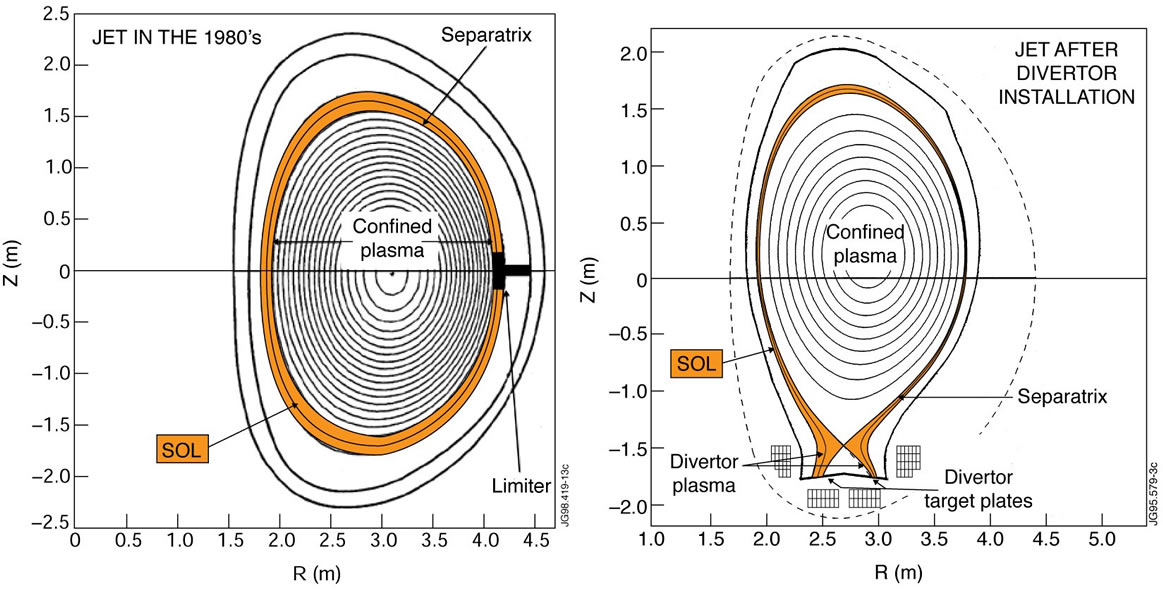
\includegraphics[height=80mm]{figures/1-limiterDivertor.jpg}
	\caption{Section verticale du tokamak JET en version limiteur
	(à gauche) et divertor (à droite). La SOL est illustrée en
	orange~\parencite{efda}.}\label{SOL}
\end{figure}
 
Typiquement, les plasmas de SOL ont une densité de
l'ordre de 10$^{19}$~m$^{-3}$ et une température inférieure à la centaine
d'électronvolts. A cette température, le plasma est presque totalement ionisé et
le champ magnétique, d'environ 3T, confine efficacement les particules dans un
mouvement cyclotronique de fréquence $\omega_{ci}\sim45$~MHz pour un proton et
$\omega_{ce}\sim80$~GHz pour un électron, toutes deux bien supérieures à la
fréquence caractéristique du transport parallèle :

\begin{equation}
\omega_\para\sim
\frac{v_{\text{T}\alpha}}{L_\para}\approx\omega_{c\alpha}\frac{\rho_{L\alpha}}{L_\para}\rightarrow
\delta=\frac{\omega_\para}{\omega_{c\alpha}}\ll1
\end{equation} 

Dans la direction perpendiculaire au champ
magnétique, les vitesses de dérive associées aux gradients transverses (dont les longueurs
typiques $L_\nabla$ de quelques centimètres sont bien supérieures aux rayon de
Larmor ionique $\rho_{Li}\approx3.10^{-4}$~m et électroniques
$\rho_{Le}\approx7.10^{-6}$~m) entraînent un transport de fréquence
caractéristique $\omega_\perp\sim v_\perp/L_\para\sim\rho_{L\alpha}
v_{\text{T}\alpha}/(L_\para L_\nabla)$ de deux ordres de grandeur inférieur à
$\omega_{c\alpha}$ :

\begin{equation}
\frac{\omega_\perp}{\omega_{c\alpha}}\approx\frac{\rho_{L\alpha}^2}{L_\para
L_\nabla}=\delta^2
\end{equation}

Malgré leur faible fréquence, ces vitesses de dérives sont à l'origine de tous
les mécanismes de micro-turbulence et jouent ainsi un rôle primordiale dans le
problème du confinement des plasmas de fusion.

\subsubsection{Vitesses de dérive électrique et diamagnétique}

Quand le degré d'ionisation du plasma est très élevé, le terme issu de
l'interaction avec le gaz peut être négligé dans l'équation du
mouvement~\eqref{1-eqBilanForce} :

\begin{equation}
\label{1-eqSOL}
 m_\alpha n_\alpha\left(\partial_t \mathbf{u_\alpha} +
(\mathbf{u_\alpha}\cdot\nabla)\mathbf{u_\alpha}\right)
={q_\alpha n_\alpha}\left(\mathbf E+\mathbf
u_\alpha\times \mathbf B\right)
-{\nabla p_\alpha}
\end{equation}

 Sous l'hypothèse de faible variation spatiale des grandeurs et des champs à
 l'échelle du rayon de Larmor, la lente évolution du système par rapport aux
 fréquences cyclotroniques permet d'effectuer un développement de l'équation du
 mouvement en fonction du petit paramètre $\delta$. En négligeant le
 mouvement cyclotronique, qui correspond à l'ordre 0 de ce développement et qui
 est de moyenne nulle sur un temp $t\sim\omega_{c\alpha}^{-1}$, la projection
 de~\eqref{1-eqSOL} perpendiculairement au champ magnétique s'écrit à l'ordre 1
 en $\delta$ :
 
 \begin{equation}
\label{1-eqSOLperp}
0
={q_\alpha n_\alpha}\left(\mathbf E+\mathbf
u_{\alpha\perp}^{(1)}\times \mathbf B\right)
-{\nabla_\perp p_\alpha}
\end{equation}

En prenant le produit vectoriel par $\mathbf B$ de cette équation, on obtient
les deux vitesses de dérive fluides principales, la vitesse de dérive électrique
$\mathbf u_E$ et la vitesse de dérive diamagnétique $\mathbf u_*$, relativement
liées aux gradients transverses de potentiel électrique $U$ et de pression
$p_\alpha$:

\begin{equation}
\mathbf u_{\alpha\perp}^{(1)}=\mathbf u_E+\mathbf u_*=\frac{\mathbf
B\times\nabla_\perp U}{B^2}-\frac{\mathbf B\times\nabla_\perp p_\alpha}{n_\alpha q_\alpha B^2}
\end{equation}

L'origine de ces vitesses de dérive est illustrée sur la
figure~\ref{1-vitessesDerive}. La dérive diamagnétique est une vitesse
purement fluide qui traduit le mouvement d'ensemble des particules, et non
une dérive individuelle de celles-ci. De ce fait, elle ne transporte que
très peu de matière en comparaison de la dérive électrique : pour s'en
convaincre, il suffit de regarder la divergence des flux issus de ces
vitesses :

\begin{equation}
\nabla\cdot\left(n_\alpha\mathbf
u_E\right)=\nabla\cdot\left(n_\alpha\frac{\mathbf B\times\nabla U}{B^2}\right)
=\nabla\frac{n_\alpha}{B}\times\nabla U\cdot \mathbf b
\end{equation}

\begin{equation}
\nabla\cdot\left(n_\alpha\mathbf
u_*\right)=\nabla\cdot\left(\frac{\mathbf B\times\nabla
p_\alpha}{q_\alpha B^2}\right)
=\frac{1}{q_\alpha}\nabla p_\alpha\times\nabla\frac{1}{B}\cdot \mathbf b
\end{equation}

La divergence du flux diamagnétique est donc nulle aux effets de courbure du
champ magnétique près. Par contre, et comme
précisé au paragraphe \S\ref{1-plasma-champMag}, la dérive diamagnétique est 
sensible à la charge des particules et est donc la seule à porter du courant.
L'influence de ce courant est fondamental dans la stabilité du plasma :

\begin{equation}
\mathbf j_*=e(n_i\mathbf u^i_*-n_e\mathbf
u^e_*)=e(\nabla(p_i+p_e)\times\mathbf B/B^2)
\end{equation}

\begin{figure}[!htbp]
    \centering
	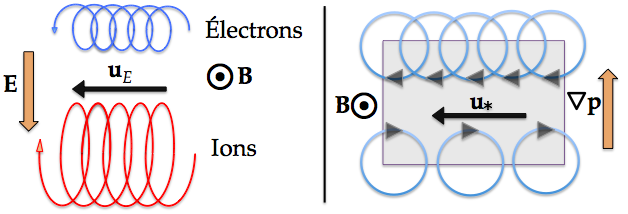
\includegraphics[height=80mm]{figures/1-vitessesDerive.jpg}
	\caption{Interprétation des vitesses de dérive électrique et diamagnétique.}
	\label{1-vitessesDerive}
\end{figure}


\subsubsection{Dérive de polarisation}

Dans le cas d'un champ électrique variant lentement dans le temps, une troisième
dérive, d'un ordre de grandeur inférieur aux dérives électrique et diamagnétique,
peut être identifiée : 

\begin{equation}
\label{1-vitessePol}
\mathbf{u}_\perp^{(2)}= \text{d}\mathbf
u_\perp^{(1)}/\text{dt}=\text{d}(\mathbf
u_E+\mathbf
u_*)/\text{dt}
\end{equation}

Par un calcul compliqué, on peut montrer que la dérivée totale de la dérive
diamagnétique est exactement compensée par la prise en compte du tenseur des
contraintes de Braginskii (les termes non-diagonaux du tenseur de
pression). L'expression de cette dérive d'ordre 2 se réduit alors à :

\begin{equation}
\label{1-vitessePol}
\mathbf{u}_\perp^{(2)}= \frac{\text{d}\mathbf
u_E}{\text{dt}}=-\frac{m_\alpha}{q_\alpha B^2}\frac{\text{d}\nabla_\perp
U}{\text{dt}}
\end{equation}

C'est la dérive de polarisation $\mathbf{u}_\perp^{(2)}=\mathbf u^\alpha_p$, qui
dérive du terme d'inertie. Bien qu'elle soit d'un ordre de grandeur inférieur aux deux autres
vitesses de dérive, la divergence du flux qui lui est associé est comparable à celle du
flux diamagnétique. Comme la dérive électrique n'a aucune influence sur
l'évolution du courant, la contribution de la dérive de polarisation est dès
lors du même ordre de grandeur que celle de la dérive diamagnétique et ne peut plus
être négligée.

\subsection{Equation de dérive-diffusion}
\label{1-transportAmbipolaire}
Les plasmas froids de décharge utilisés dans l'industrie et la recherche n'ont
en général qu'un faible degré d'ionisation $\alpha<$1\% et la dynamique des
espèces y est dominée par la perte de quantité de mouvement liée à l'ionisation
et aux collisions avec le gaz. Pour modéliser ce type de plasma, la prise en
compte du terme collisionnel dans l'équation du mouvement est essentielle.
En l'absence de champ magnétique, le rapport d'échelle entre le libre parcours moyen des particules
et la taille du plasma $\lambda_\alpha\ll L$ permet de simplifier l'équation du
mouvement en négligeant les termes d'inertie, relativement faibles\footnote{Les
termes inertiels peuvent être négligés quand la vitesse fluide $\mathbf u$ est
subsonique : $\mathbf u$ vérifie alors $\mathbf u\ll \left<v\right>/K_n$, où
$K_n=\lambda/L$ est le nombre de Knudsen et $$\nu \mathbf u=\frac{
\left<v\right>\mathbf u}{\lambda}\gg \frac{u^2}{\lambda}K_n=\frac{u^2}{L}\sim
\mathbf u\cdot\nabla\mathbf u$$} par rapport au terme collisionnel :

\begin{equation}
\label{1-eqDriftDif}
n_\alpha\mathbf u_\alpha=\frac{q_\alpha}{\nu_\alpha m_\alpha}n_\alpha\mathbf
E-\frac{\nabla\left(n_\alpha eT_\alpha\right)}{\nu_\alpha
m_\alpha}\equiv\frac{q_\alpha}{|q_\alpha|}\mu_\alpha n_\alpha\mathbf
E-{\nabla\left(D_\alpha n_\alpha\right)}
\end{equation}

C'est l'équation de dérive-diffusion, avec les coefficients de
transport $\mu_\alpha$ et $D_\alpha$, tous deux
inversement proportionnels à la fréquence de collision $\nu_\alpha$ (donc à la
densité de gaz), et reliés par la relation d'Einstein :

\begin{equation}
\label{1-EinsteinRelation}
D_\alpha/\mu_\alpha=T_\alpha
\end{equation}

\begin{itemize}
  \item la mobilité, définie par $\mu_\alpha=q_\alpha/\nu_\alpha m_\alpha$,
  mesure la disposition d'une espèce à laisser passer le courant au sein d'un milieu
  \item la diffusion, de coefficient $D_\alpha=eT_\alpha/\nu_\alpha m_\alpha$,
  représente la tendance naturelle d'un système à rendre homogène sa densité de particule sous l'effet
  de l'agitation thermique.
\end{itemize}

En combinant \eqref{1-eqDriftDif} avec l'équation de continuité
\eqref{1-eqContinuite}, on obtient une équation d'évolution de la densité
constituée d'une loi d'Ohm et d'une loi de Fick :
 
\begin{equation}
\label{1-eqDriftDifContinuite}
\partial_t
n_\alpha=\nabla\cdot(\underbrace{\frac{q_\alpha}{|q_\alpha|}\mu_\alpha n_\alpha\mathbf E}_\text{Loi d'Ohm}+\underbrace{D_\alpha{\nabla n_\alpha}}_\text{Loi
de Fick})+S_\alpha
\end{equation}

Dans des plasmas de décharge collisionnels, à partir de la source d'ionisation,
les électrons ont tendance à se déplacer beaucoup plus rapidement que les ions
du fait de leur faible masse et de leur température. Cette différence de
mobilité entraîne l'apparition d'un champ électrique dit "ambipolaire"
$\mathbf E_a$, faisant dériver les ions et les électrons ensembles et
systématiquement dirigé dans le sens opposé du gradient de densité afin de
limiter la diffusion des électrons et accélérer les ions. En ne considérant
qu'une seule espèce ionique, on trouve son expression en cherchant le champ
correspondant à un courant nul :
 
\begin{equation}
\label{1-eqEAmb}
\mathbf j=0 \Rightarrow \mathbf E=\mathbf
E_a=\frac{D_i-D_e}{\mu_i+\mu_e}\frac{\nabla n}{n}
\end{equation}

A l'interface entre les parois et le plasma, une gaine positive se
forme et enferme les électrons dans un puit de potentiel. Ce phénomène, en plus
des collisions, permet une isotropisation rapide de la fonction de distribution
des électrons, qui peuvent alors être considérés en équilibre de Boltzmann.
Les ions, quant-à-eux, ont une durée de vie de l'ordre de
$\nu_\text{iz}\puissance{-1}$ : depuis leur zone de création, ils sont
continuement accélérés par le champ ambipolaire jusqu'à être perdus à la paroi
où ils se recombinent. La théorie classique des gaines prédit qu'à l'équilibre,
la densité diminue d'un facteur 2 et la chute de potentiel ambipolaire est
de l'ordre de $T_e/2$ (cf. \S\ref{1-gaines}.

\subsection{Equation de dérive-diffusion magnétisée}
\label{1-deriveDiffMag}
L'utilisation d'un champ magnétique dans un plasma permet de contrôler en partie
le transport des particules et d'obtenir des configurations favorables pour
diverses applications. Cependant, la prise en compte du terme de Laplace dans
\eqref{1-eqBilanForce} impose une forte anisotopie dans le système, ce qui
complexifie considérablement les phénomènes de transport : en
négligeant l'inertie, on peut considérer \eqref{1-eqBilanForce} comme une
équation algébrique d'inconnue $\mathbf u$ qui s'écrit sous une forme
tensorielle de l'équation de dérive-diffusion :

\begin{equation}
\label{1-eqDriftDif}
n_\alpha\mathbf u_\alpha=\frac{q_\alpha}{|q_\alpha|}\mu_\alpha
n_\alpha\left(\mathbf E+\mathbf u_\alpha\times\mathbf
B\right)-\nabla\left(D_\alpha n_\alpha\right)\equiv
\frac{q_\alpha}{|q_\alpha|} n_\alpha\boldsymbol{\mu}_\alpha\cdot \mathbf
E-{\nabla\left(\mathbf{D}_\alpha n_\alpha\right)}
\end{equation}

où la mobilité $\boldsymbol{\mu}_\alpha$ et la diffusion $\mathbf{D}_\alpha$
sont devenus des tenseurs d'ordre 2 :

\begin{align}
\boldsymbol{\mu}_\alpha =
 \begin{pmatrix}
  \mu_{\alpha\perp} & \mu_{\alpha\times} & 0 \\
  \mu_{\alpha\times} & \mu_{\alpha\perp} & 0 \\
  0  & 0  & \mu_{\alpha\para} 
 \end{pmatrix}\;\;\;\;\text{et}\;\;\;\;
 \mathbf D_\alpha =
 \begin{pmatrix}
  D_{\alpha\perp} & D_{\alpha\times} & 0 \\
  D_{\alpha\times} & D_{\alpha\perp} & 0 \\
  0  & 0  & D_{\alpha\para} 
 \end{pmatrix}
\end{align}

Dans la direction parallèle au champ magnétique, les coefficients de mobilité et
de diffusion sont inchangés
$\mu_{\alpha\para}=\mu_{\alpha}=q_\alpha/m_\alpha\nu_\alpha$ et
$D_{\alpha\para}=D_\alpha=eT_\alpha/m_\alpha\nu_\alpha$. Les coefficients de la
direction perpendiculaire font quant à eux apparaître le paramètre de Hall
$h_\alpha=\omega_{c\alpha}/\nu_\alpha$ :

\begin{align}
\mu_{\alpha\perp}=\frac{1}{1+h_\alpha^2}\mu_\alpha\;\;\;\;\;\;\;\;
\;\;\;\;D_{\alpha\perp}=\frac{1}{1+h_\alpha^2}D_\alpha
\end{align}
\begin{align}
\mu_{\alpha\times}=\frac{h_\alpha}{1+h_\alpha^2}\mu_\alpha\;\;\;\;
\;\;\;\;\;\;\;\;D_{\alpha\times}=\frac{h_\alpha}{1+h_\alpha^2}D_\alpha
\end{align}

Quand $h_\alpha=0$, les tenseurs sont diagonaux et isotropes. Ensuite, plus le
facteur de hall augmente, plus le transport dans les directions transverses se
réduit :
les coefficients indicés avec le symbole perpendiculaire sont inversement
proportionnels au carré du champ magnétique $\mu_{\alpha\perp},
D_{\alpha\perp}\propto B\puissance{-2}$ ; à partir de $h_\alpha=1$, le
transport croisé commence à dominer sur le transport collisionnel et devient proportionnel à
$B\puissance{-1}$. Cette loi de puissance que suit le transport par rapport au
champ magnétique est souvent interprétée comme la signature d'un transport
anormal, mais apparaît naturellement dans les équations à travers les
coefficients $\mu_{\alpha\times}$ et $D_{\alpha\times}$.



%\bibliographystyle{apalike}
%\bibliography{biblio}
\end{refsection}

